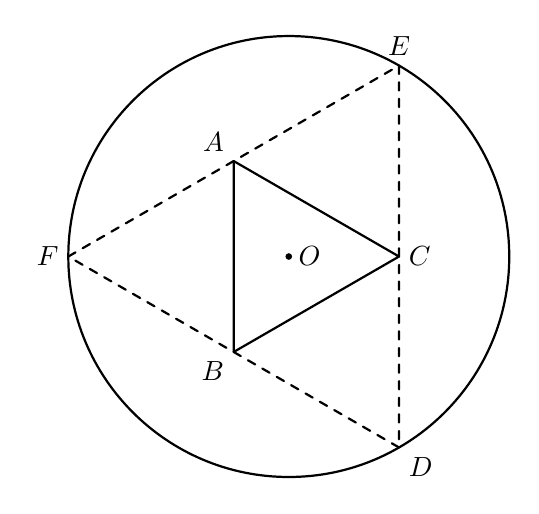
\begin{tikzpicture}[scale=1.0, line cap=round, line join=round]
\usetikzlibrary{calc}
\def\R{2.8}

\coordinate (O) at (0,0);
\coordinate (E) at (60:\R);
\coordinate (D) at (-60:\R);
\coordinate (F) at (180:\R);

\coordinate (A) at ($(F)!0.5!(E)$);
\coordinate (B) at ($(F)!0.5!(D)$);
\coordinate (C) at ($(E)!0.5!(D)$);

\draw[thick] (O) circle (\R);

\draw[dashed, thick] (F)--(E)--(D)--cycle;

\draw[thick] (A)--(B)--(C)--cycle;

\fill (O) circle (1.2pt);
\node[right] at (O) {$O$};

\node[above] at (E) {$E$};
\node[below right] at (D) {$D$};
\node[left] at (F) {$F$};

\node[above left] at (A) {$A$};
\node[below left] at (B) {$B$};
\node[right] at (C) {$C$};
\end{tikzpicture}